% Section : Optimisations Algorithmiques et Système

% Frame 1 : Algorithme Glouton Exact
\begin{frame}{ Algorithme Glouton (Exact Greedy Split)}
    \begin{columns}[T]
        \begin{column}{0.5\textwidth}
            \begin{block}{Principe}
                \small
                L'algorithme parcourt \textbf{toutes} les valeurs triées de chaque caractéristique pour trouver le split optimal.
            \end{block}
            \scriptsize
            \begin{itemize}
                \item Pour chaque variable, on trie les données.
                \item On scanne de gauche à droite.
                \item On calcule le Gain à chaque intervalle.
            \end{itemize}
            \vspace{0.2cm}
            \begin{alertblock}{Limitation}\scriptsize
                Extrêmement précis mais \textbf{coûteux} en mémoire et en temps sur des jeux de données massifs (Big Data).
            \end{alertblock}
        \end{column}
        \begin{column}{0.48\textwidth}
            \centering
            \textbf{Scan des Points}\\[0.2cm]
            \resizebox{\columnwidth}{!}{
            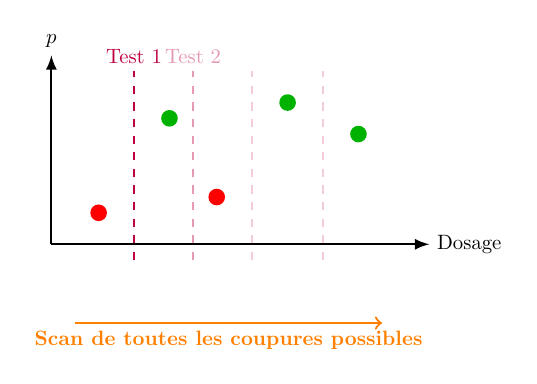
\begin{tikzpicture}[x=0.6cm, y=2cm, every node/.style={scale=0.75}]
                % Axes
                \draw[->, thick, -latex] (0,0) -- (8,0) node[right] {Dosage};
                \draw[->, thick, -latex] (0,0) -- (0,1.2) node[above] {$p$};
                
                % Points
                \fill[red] (1,0.2) circle (3pt);
                \fill[green!70!black] (2.5,0.8) circle (3pt);
                \fill[red] (3.5,0.3) circle (3pt);
                \fill[green!70!black] (5,0.9) circle (3pt);
                \fill[green!70!black] (6.5,0.7) circle (3pt);
                
                % Scan line
                \draw[thick, purple, dashed] (1.75, -0.1) -- (1.75, 1.1) node[above] {Test 1};
                \draw[thick, purple, dashed, opacity=0.4] (3.0, -0.1) -- (3.0, 1.1) node[above, opacity=0.4] {Test 2};
                \draw[thick, purple, dashed, opacity=0.2] (4.25, -0.1) -- (4.25, 1.1);
                \draw[thick, purple, dashed, opacity=0.2] (5.75, -0.1) -- (5.75, 1.1);
                
                % Arrows
                \draw[thick, ->, orange] (0.5, -0.5) -- (7, -0.5) node[midway, below] {\textbf{Scan de toutes les coupures possibles}};
            \end{tikzpicture}}
        \end{column}
    \end{columns}
\end{frame}


% IMAGE : Histogram-based splits
\begin{frame}{ Histogram-based Split Finding — Illustration}
\begin{figure}
    \centering
    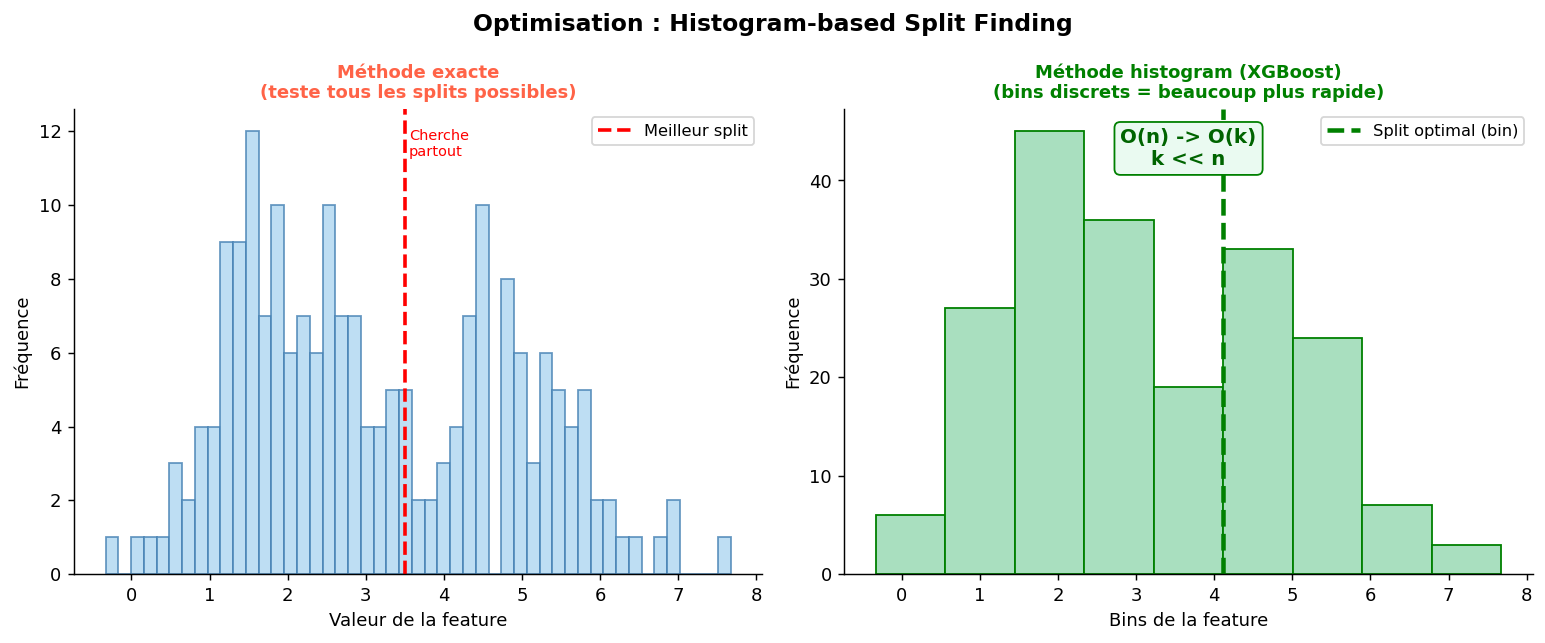
\includegraphics[width=0.95\linewidth]{imagens/xgb_histogram_split.png}
    \caption{XGBoost remplace la recherche exacte par des bins discrets : $O(n) \rightarrow O(k)$ avec $k \ll n$.}
\end{figure}
\end{frame}

% Frame 5 : Apprentissage Parallèle
\begin{frame}{ Apprentissage Parallèle (Column Blocks)}
    \begin{block}{Innovation : Stockage par Blocs de Colonnes}
        \small
        XGBoost stocke les données dans une structure en mémoire appelée \textbf{Block}.
    \end{block}
    
    \scriptsize
    \begin{itemize}
        \item Les données sont pré-triées par colonne avant l'entraînement.
        \item Chaque colonne peut être traitée par un cœur CPU différent \textbf{en parallèle}.
        \item Réduit drastiquement le coût du tri (l'étape la plus lente du boosting).
    \end{itemize}

    \centering
    \resizebox{0.8\textwidth}{!}{
    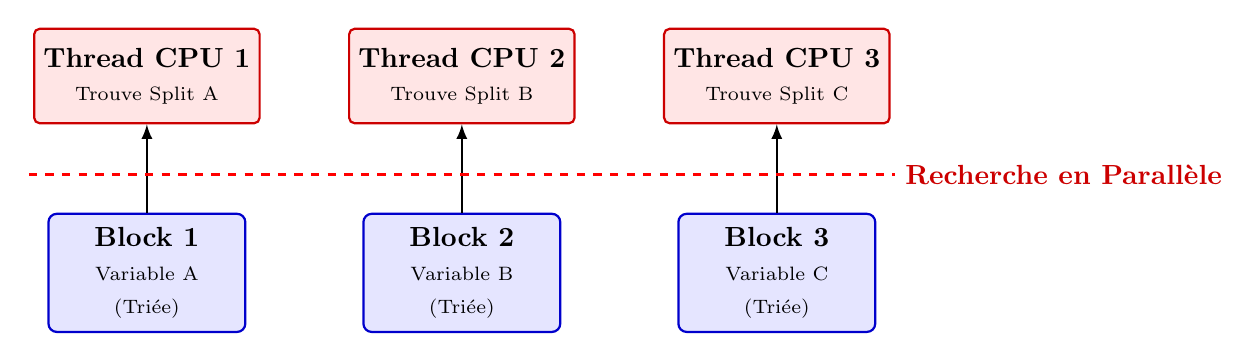
\begin{tikzpicture}[
        block/.style={rectangle, draw, rounded corners=3pt, thick, align=center, minimum height=1.5cm},
        cpu/.style={rectangle, draw=red!80!black, fill=red!10, thick, rounded corners=2pt, minimum width=2.5cm, minimum height=1.2cm, align=center}
    ]
        % Block Memory
        \node[block, fill=blue!10, draw=blue!80!black, minimum width=2.5cm] (v1) at (0,0) {\textbf{Block 1} \\ \scriptsize Variable A \\ \scriptsize (Triée)};
        \node[block, fill=blue!10, draw=blue!80!black, minimum width=2.5cm] (v2) at (4,0) {\textbf{Block 2} \\ \scriptsize Variable B \\ \scriptsize (Triée)};
        \node[block, fill=blue!10, draw=blue!80!black, minimum width=2.5cm] (v3) at (8,0) {\textbf{Block 3} \\ \scriptsize Variable C \\ \scriptsize (Triée)};
        
        % CPUs
        \node[cpu] (c1) at (0, 2.5) {\textbf{Thread CPU 1} \\ \scriptsize Trouve Split A};
        \node[cpu] (c2) at (4, 2.5) {\textbf{Thread CPU 2} \\ \scriptsize Trouve Split B};
        \node[cpu] (c3) at (8, 2.5) {\textbf{Thread CPU 3} \\ \scriptsize Trouve Split C};
        
        % Arrows
        \draw[<->, thick, -latex] (v1.north) -- (c1.south);
        \draw[<->, thick, -latex] (v2.north) -- (c2.south);
        \draw[<->, thick, -latex] (v3.north) -- (c3.south);
        
        % Parallelism line
        \draw[thick, red, dashed] (-1.5, 1.25) -- (9.5, 1.25) node[right, red!80!black] {\textbf{Recherche en Parallèle}};
    \end{tikzpicture}}
\end{frame}


% Frame 3 : Weighted Quantile Sketch
\begin{frame}{ Esquisse de Quantiles Pondérés}
    \begin{block}{Innovation : Weighted Quantile Sketch}
        \small
        XGBoost ne découpe pas les "buckets" de manière uniforme. Il utilise la \textbf{Hessienne ($h_i$)} comme poids.
    \end{block}
    
    \scriptsize
    \begin{itemize}
        \item Rappel : En classification, $h_i = p_i(1-p_i)$ est la \textbf{confiance} ou la variance.
        \item Les points avec une forte Hessienne (incertitude) méritent des bacs plus précis.
        \item \textbf{Sketch} : Algorithme permettant de trouver ces quantiles sur des données massives avec peu de mémoire.
    \end{itemize}

    \centering
    \resizebox{0.8\textwidth}{!}{
    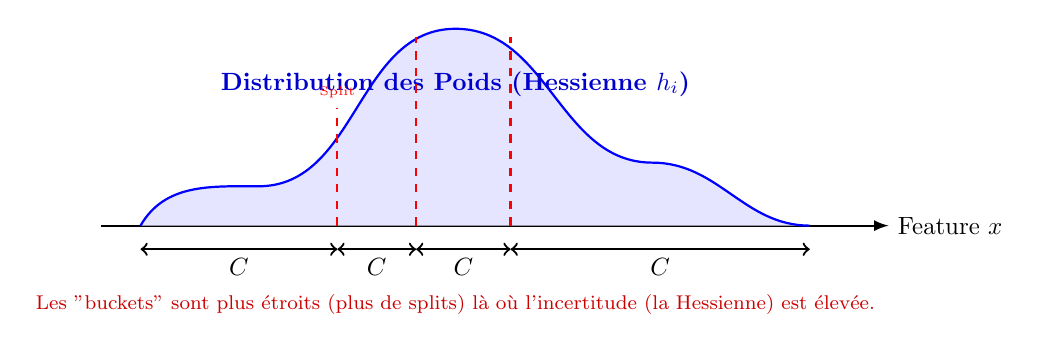
\begin{tikzpicture}[every node/.style={scale=0.9}]
        % Axe
        \draw[->, thick, -latex] (0,0) -- (10,0) node[right] {Feature $x$};
        
        % Densite de Hessienne
        \draw[thick, blue, fill=blue!10, smooth] (0.5,0) to[out=60, in=180] (2, 0.5) to[out=0, in=180] (4.5, 2.5) to[out=0, in=180] (7, 0.8) to[out=0, in=180] (9,0);
        \node[blue!80!black] at (4.5, 1.8) {\textbf{Distribution des Poids (Hessienne $h_i$)}};
        
        % Decoupage des quantiles proportionnels a l'aire (Hessienne)
        % Zone 1 : faible aire, donc large intervalle x
        \draw[thick, dashed, red] (3.0, 0) -- (3.0, 1.5) node[above] {\tiny Split};
        \draw[<->, thick] (0.5, -0.3) -- (3.0, -0.3) node[midway, below] {$C$};
        
        % Zone 2 : forte aire, intervalle etroit
        \draw[thick, dashed, red] (4.0, 0) -- (4.0, 2.4);
        \draw[<->, thick] (3.0, -0.3) -- (4.0, -0.3) node[midway, below] {$C$};
        
        % Zone 3 : forte aire
        \draw[thick, dashed, red] (5.2, 0) -- (5.2, 2.4);
        \draw[<->, thick] (4.0, -0.3) -- (5.2, -0.3) node[midway, below] {$C$};
        
        % Zone 4 : faible aire, large intervalle
        \draw[thick, dashed, red] (9.0, 0) -- (9.0, 0.0);
        \draw[<->, thick] (5.2, -0.3) -- (9.0, -0.3) node[midway, below] {$C$};
        
        % Commentaire
        \node[red!80!black] at (4.5, -1.0) {\footnotesize Les "buckets" sont plus étroits (plus de splits) là où l'incertitude (la Hessienne) est élevée.};
    \end{tikzpicture}}
\end{frame}

% Frame 4 : Parcimonie (1/3)
\begin{frame}{Parcimonie (1/3) : Valeurs Manquantes}
    \begin{columns}[T]
        \begin{column}{0.45\textwidth}
            \textbf{Réalité des données :}
            \vspace{0.1cm}
            
            \begin{table}
                \centering
                \scriptsize
                \begin{tabular}{|c|c|c|c|}
                    \hline
                    \textbf{ID} & \textbf{Dosage} & \textbf{Effic.} ($y_i$) & \textbf{Résidu} ($r_i$) \\
                    \hline
                    1 & 2 & 0 & -0.5 \\
                    2 & 8 & 1 & +0.5 \\
                    3 & \textbf{NaN} & 1 & +0.5 \\
                    4 & 18 & 0 & -0.5 \\
                    \hline
                \end{tabular}
                \caption{\scriptsize $p_0=0.5 \implies r_i = y_i - 0.5$. Donnée manquante pour l'ID 3.}
            \end{table}
            
            \begin{alertblock}{Le défi}
                \scriptsize
                Les algorithmes classiques rejettent les lignes avec des valeurs manquantes ou nécessitent une imputation ($moyenne$, $médiane$).
            \end{alertblock}
        \end{column}
        
        \begin{column}{0.55\textwidth}
            \begin{block}{L'approche native de XGBoost}
                \small
                XGBoost traite la parcimonie (données vides, zéros, NaN) de manière \textbf{unifiée} et \textbf{apprise}.
                
                \vspace{0.2cm}
                \begin{itemize}
                    \item \textbf{Aucune imputation nécessaire} : On ne "devine" pas la valeur.
                    \item \textbf{Direction par défaut} : On apprend quel chemin (Gauche ou Droit) est le meilleur pour les données manquantes.
                \end{itemize}
            \end{block}
        \end{column}
    \end{columns}
\end{frame}

\begin{frame}{ Parcimonie (2/4) : Test de la Coupure $< 5$}
    \begin{block}{Étape 1 : Tester la coupure valide $< 5$}
        \small
        XGBoost calcule la pertinence de la coupure (Gain) sur les données observées, puis teste l'affectation du \textbf{\textit{NaN}} à Gauche et à Droite.
    \end{block}

    \begin{columns}[T]
        \begin{column}{0.5\textwidth}
            \centering
            \textbf{\scriptsize Scénario A : $NaN$ à GAUCHE}
            \vspace{0.2cm}
            
            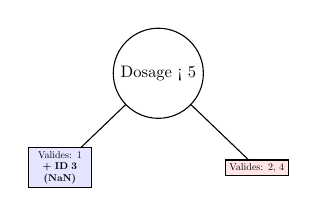
\begin{tikzpicture}[
                level 1/.style={sibling distance=2.5cm, level distance=1.2cm},
                every node/.style={circle, draw, align=center, scale=0.6},
                leaf/.style={rectangle, draw, fill=green!10, text width=2cm, scale=0.6}
            ]
                \node {Dosage < 5}
                    child {node[leaf, fill=blue!10] {Valides: 1 \\ \textbf{+ ID 3 (NaN)}}}
                    child {node[leaf, fill=red!10] {Valides: 2, 4}};
            \end{tikzpicture}
            
            \vspace{0.2cm}
            \scriptsize Gain$_A$ = $0.00$
        \end{column}
        
        \begin{column}{0.5\textwidth}
            \centering
            \textbf{\scriptsize Scénario B : $NaN$ à DROITE}
            \vspace{0.2cm}
            
            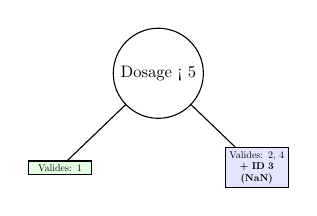
\begin{tikzpicture}[
                level 1/.style={sibling distance=2.5cm, level distance=1.2cm},
                every node/.style={circle, draw, align=center, scale=0.6},
                leaf/.style={rectangle, draw, fill=green!10, text width=2cm, scale=0.6}
            ]
                \node {Dosage < 5}
                    child {node[leaf] {Valides: 1}}
                    child {node[leaf, fill=blue!10] {Valides: 2, 4 \\ \textbf{+ ID 3 (NaN)}}};
            \end{tikzpicture}
            
            \vspace{0.2cm}
            \scriptsize Gain$_B$ = \textbf{1.33}
        \end{column}
    \end{columns}
\end{frame}

\begin{frame}{ Parcimonie (3/4) : Test de la Coupure $< 13$}
    \begin{block}{Étape 2 : Tester l'autre coupure valide $< 13$}
        \small
        Il répète l'opération pour la coupure suivante (séparant ID 2 et 4).
    \end{block}

    \begin{columns}[T]
        \begin{column}{0.5\textwidth}
            \centering
            \textbf{\scriptsize Scénario C : $NaN$ à GAUCHE}
            \vspace{0.2cm}
            
            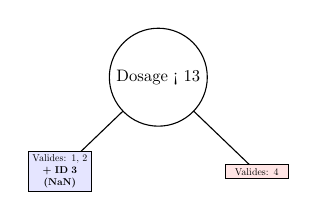
\begin{tikzpicture}[
                level 1/.style={sibling distance=2.5cm, level distance=1.2cm},
                every node/.style={circle, draw, align=center, scale=0.6},
                leaf/.style={rectangle, draw, fill=green!10, text width=2cm, scale=0.6}
            ]
                \node {Dosage < 13}
                    child {node[leaf, fill=blue!10] {Valides: 1, 2 \\ \textbf{+ ID 3 (NaN)}}}
                    child {node[leaf, fill=red!10] {Valides: 4}};
            \end{tikzpicture}
            
            \vspace{0.2cm}
            \scriptsize Gain$_C$ = \textbf{1.33}
        \end{column}
        
        \begin{column}{0.5\textwidth}
            \centering
            \textbf{\scriptsize Scénario D : $NaN$ à DROITE}
            \vspace{0.2cm}
            
            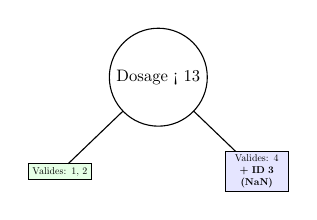
\begin{tikzpicture}[
                level 1/.style={sibling distance=2.5cm, level distance=1.2cm},
                every node/.style={circle, draw, align=center, scale=0.6},
                leaf/.style={rectangle, draw, fill=green!10, text width=2cm, scale=0.6}
            ]
                \node {Dosage < 13}
                    child {node[leaf] {Valides: 1, 2}}
                    child {node[leaf, fill=blue!10] {Valides: 4 \\ \textbf{+ ID 3 (NaN)}}};
            \end{tikzpicture}
            
            \vspace{0.2cm}
            \scriptsize Gain$_D$ = $0.00$
        \end{column}
    \end{columns}
\end{frame}

% Frame 6 : Parcimonie (3/3)
\begin{frame}{Parcimonie (4/4) : Arbre Sparsity-Aware Final}
    \begin{columns}[T]
        \begin{column}{0.45\textwidth}
            \textbf{Résultat de l'apprentissage :}
            \vspace{0.3cm}
            
            \begin{itemize}
                \item Le modèle a remarqué que les patients sans donnée de dosage (ID 3) ont souvent une efficacité positive ($y=1$).
                \item La direction par défaut suivra donc le nœud qui mène aux prédictions positives.
            \end{itemize}
        \end{column}
        
        \begin{column}{0.55\textwidth}
            \centering
            \begin{block}{Arbre avec directions par défaut}
                \vspace{0.5cm}
                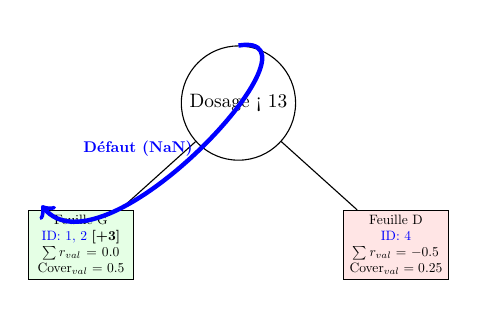
\begin{tikzpicture}[
                    level 1/.style={sibling distance=4cm, level distance=1.8cm},
                    every node/.style={circle, draw, align=center, scale=0.7},
                    leaf/.style={rectangle, draw, fill=green!10, text width=2.5cm, scale=0.7}
                ]
                \node (root) {Dosage < 13}
                    child {node[leaf] {Feuille G \\ \textcolor{blue}{ID: 1, 2} \textbf{[+3]} \\ $\sum r_{val} = 0.0$ \\ Cover$_{val} = 0.5$}}
                    child {node[leaf, fill=red!10] {Feuille D \\ \textcolor{blue}{ID: 4} \\ $\sum r_{val} = -0.5$ \\ Cover$_{val} = 0.25$}};
                
                % Fleche epaisse pour le defaut
                \draw[->, ultra thick, blue, bend right=30] (root.north) to[out=150, in=90] node[midway, left, scale=0.8, draw=none] {\textbf{Défaut (NaN)}} (-2.5, -1.3);
                \end{tikzpicture}
            \end{block}
            
            \vspace{0.2cm}
            \scriptsize \textit{La flèche bleue indique le chemin automatique \\ pour toute nouvelle donnée manquante.}
        \end{column}
    \end{columns}
\end{frame}


% Frame 6 : Accès Optimisé au Cache
\begin{frame}{ Accès Optimisé au Cache}
    \begin{block}{Cache-Aware Prefetching}
        \small
        Les accès mémoire non contigus ralentissent le CPU. XGBoost utilise un \textbf{Buffer interne}.
    \end{block}
    
    \scriptsize
    \begin{itemize}
        \item Les gradients sont récupérés par blocs pour tenir dans le \textbf{L1/L2 Cache}.
        \item Évite les "Cache Miss" (quand le CPU attend la RAM).
        \item Crucial pour la performance "Extreme" sur processeurs modernes.
    \end{itemize}

    \centering
    \resizebox{0.8\textwidth}{!}{
    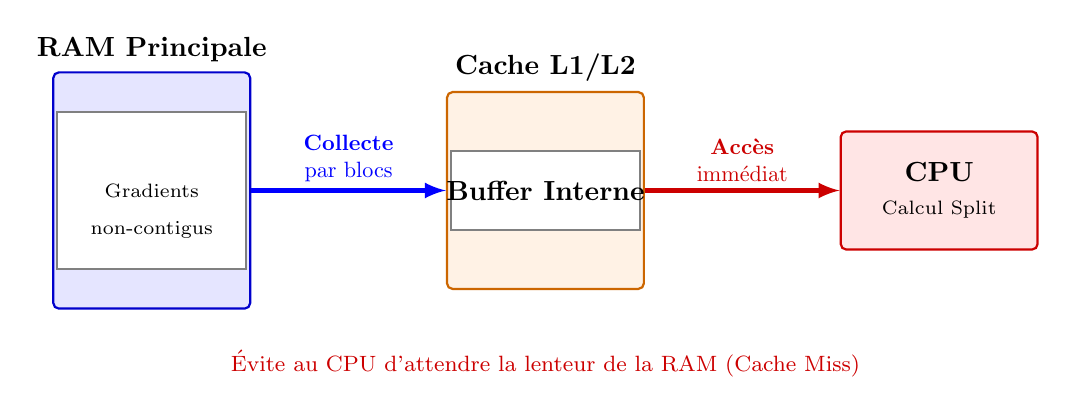
\begin{tikzpicture}[
        mem/.style={rectangle, draw=blue!80!black, fill=blue!10, thick, minimum width=2.5cm, minimum height=3cm, rounded corners=2pt, align=center},
        cache/.style={rectangle, draw=orange!80!black, fill=orange!10, thick, minimum width=2.5cm, minimum height=2.5cm, rounded corners=2pt, align=center},
        cpu/.style={rectangle, draw=red!80!black, fill=red!10, thick, minimum width=2.5cm, minimum height=1.5cm, rounded corners=2pt, align=center}
    ]
        % RAM
        \node[mem] (ram) at (0,0) {};
        \node[above] at (ram.north) {\textbf{RAM Principale}};
        \draw[fill=white, draw=gray, thick] (-1.2, -1) rectangle (1.2, 1);
        \node at (0,0) {\scriptsize Gradients};
        \node at (0,-0.5) {\scriptsize non-contigus};
        
        % L1/L2
        \node[cache] (cache) at (5,0) {};
        \node[above] at (cache.north) {\textbf{Cache L1/L2}};
        \draw[fill=white, draw=gray, thick] (3.8, -0.5) rectangle (6.2, 0.5);
        \node at (5,0) {\textbf{Buffer Interne}};
        
        % CPU
        \node[cpu] (cpu) at (10,0) {\textbf{CPU} \\ \scriptsize Calcul Split};
        
        % Connections
        \draw[->, ultra thick, blue, -latex] (ram.east) -- (cache.west) node[midway, above, align=center, scale=0.8] {\textbf{Collecte} \\ par blocs};
        \draw[->, ultra thick, red!80!black, -latex] (cache.east) -- (cpu.west) node[midway, above, align=center, scale=0.8] {\textbf{Accès} \\ immédiat};
        
        % Label
        \node[text=red!80!black, align=center] at (5, -2.2) {\footnotesize Évite au CPU d'attendre la lenteur de la RAM (Cache Miss)};
    \end{tikzpicture}}
\end{frame}

% Frame 7 : Calculs Hors-Mémoire (Out-of-Core)
\begin{frame}{ Calculs Hors-Mémoire (Principe)}
    \begin{block}{Traitement du Big Data}
        \small
        Pour les données plus grandes que la RAM, XGBoost optimise les accès disque.
    \end{block}
    
    \vspace{0.3cm}
    \begin{itemize}
        \item \textbf{Compression par blocs} : Les données sur le disque sont compressées (algorithme LZ4 très performant).
        \item \textbf{Décompression à la volée} : Un thread indépendant du CPU s'occupe de la décompression avant que le modèle n'en ait besoin.
        \item \textbf{Sharding} : Les données sont réparties sur plusieurs disques pour paralléliser les lectures (I/O) et maximiser le débit.
    \end{itemize}
\end{frame}

\begin{frame}{ Calculs Hors-Mémoire (Architecture)}
    \centering
    \vspace{0.5cm}
    \resizebox{0.95\linewidth}{!}{
    \begin{tikzpicture}[
        disk/.style={cylinder, draw=gray!80!black, fill=gray!20, thick, shape border rotate=90, minimum width=2cm, minimum height=2.5cm, align=center},
        block/.style={rectangle, draw=orange!80!black, fill=orange!10, thick, rounded corners=2pt, minimum width=3cm, minimum height=1.5cm, align=center}
    ]
        % Disks
        \node[disk] (d1) at (0, 2.0) {\textbf{Disque 1} \\ \scriptsize Blocs compressés \\ \scriptsize (LZ4)};
        \node[disk] (d2) at (0, -2.0) {\textbf{Disque 2} \\ \scriptsize Blocs compressés \\ \scriptsize (LZ4)};
        
        % Threads deflate
        \node[block] (t1) at (4.5, 2.0) {\textbf{Thread CPU Indépendant} \\ \scriptsize Décompression à la volée};
        \node[block] (t2) at (4.5, -2.0) {\textbf{Thread CPU Indépendant} \\ \scriptsize Décompression à la volée};
        
        % RAM
        \node[rectangle, draw=green!80!black, fill=green!10, thick, rounded corners=2pt, minimum height=6cm, minimum width=3.5cm, align=center] (ram) at (10, 0) {\textbf{RAM Principale} \\ \vspace{0.2cm} \\ \scriptsize Algorithme \\ \scriptsize d'entraînement \\ \scriptsize (XGBoost)};
        
        % Arrows
        \draw[->, ultra thick, gray, -latex] (d1.east) -- (t1.west) node[midway, above] {Lecture};
        \draw[->, ultra thick, gray, -latex] (d2.east) -- (t2.west) node[midway, above, text width=2cm, align=center, yshift=-0.2cm] {Sharding};
        
        \draw[->, ultra thick, blue, -latex] (t1.east) -- (ram.150);
        \draw[->, ultra thick, blue, -latex] (t2.east) -- (ram.210);
    \end{tikzpicture}}
\end{frame}
